\documentclass[12pt,letterpaper]{article}
\usepackage[utf8]{inputenc}
\usepackage[spanish]{babel}
\usepackage{graphicx}
\usepackage[left=2cm,right=2cm,top=2cm,bottom=2cm]{geometry}
\usepackage{graphicx} % figuras
% \usepackage{subfigure} % subfiguras
\usepackage{float} % para usar [H]
\usepackage{amsmath}
%\usepackage{txfonts}
\usepackage{stackrel} 
\usepackage{multirow}
\usepackage{enumerate} % enumerados
\renewcommand{\labelitemi}{$-$}
\renewcommand{\labelitemii}{$\cdot$}
% \author{}
% \title{Caratula}
\begin{document}

% Fancy Header and Footer
% \usepackage{fancyhdr}
% \pagestyle{fancy}
% \cfoot{}
% \rfoot{\thepage}
%

% \usepackage[hidelinks]{hyperref} % CREA HYPERVINCULOS EN INDICE

% \author{}
\title{Caratula}

\begin{titlepage}
\begin{center}
\large{UNERSIDAD PRIVADA DE TACNA}\\
\vspace*{-0.025in}
\begin{figure}[htb]
\begin{center}

\includegraphics[width=8cm]{./Imagenes/logo}
\end{center}
\end{figure}
\vspace*{0.15in}
INGENIERIA DE SISTEMAS  \\

\vspace*{0.5in}
\begin{large}
TITULO:\\
\end{large}

\vspace*{0.1in}
\begin{Large}
\textbf{Trabajo Final de Unidad I} \\
\end{Large}

\vspace*{0.3in}
\begin{Large}
\textbf{CURSO:} \\
\end{Large}

\vspace*{0.1in}
\begin{large}
BASE DE DATOS II\\
\end{large}

\vspace*{0.3in}
\begin{Large}
\textbf{DOCENTE(ING):} \\
\end{Large}

\vspace*{0.1in}
\begin{large}
 Patrick Cuadros Quiroga\\
\end{large}

\vspace*{0.2in}
\vspace*{0.1in}
\begin{large}
Integrantes: \\
\begin{flushleft}
Alfaro Musaja Jhosmell Gyno \hfill	(2015053223) \\
Perez Mamani Nilton Edy \hfill	(2015053233) \\

Perez Mamani Nilton Edy \hfill	(2015053233) \\


\end{flushleft}
\end{large}
\end{center}

\end{titlepage}


\tableofcontents % INDICE
\thispagestyle{empty} % INDICE SIN NUMERO
\newpage
\setcounter{page}{1} % REINICIAR CONTADOR DE PAGINAS DESPUES DEL INDICE

\section{PROBLEMA} 

\begin{enumerate}[1.]
    
    Las bibliotecas siempre han estado al tanto de nuevas tecnologías que permitan desempeñar de una manera mejor su papel de brindar información. Además las infraestructuras informáticas y de telecomunicaciones que actualmente poseen diversas instituciones tanto públicas como privadas, permiten pensar en llevar a otro nivel el uso de estas.
    \\ Actualmente se utliza de manera manual haciéndolo en un determinado tiempo de espera prolongado afectando al estudiante, el encargado presenta estos problemas al momento de la búsqueda de un libro, por autor, editorial y fecha de publicación por ser manejable, no dan rapidez ni solución concreta, cabe rescatar que no poseen un registro de cada libro que se pueda llevar un estudiante de la institución, ni una organización de cada asignatura de manera automatizada, a la llegada de un nuevo libro no contiene anotaciones para poder implementar dicho libro a la biblioteca , no contener un sistema automatizado acapara mucha información ya que se desperdicia.
\\ La motivación principal de este proyecto es por lo tanto mejorar el servicio de préstamo de libros y que produzca en una mayor agilidad y eficacia tanto para el usuario como el empleado de estos servicios bibliotecarios.


\end{enumerate} 


\section{MARCO TEORICO} 

\begin{enumerate}[1.]
	\item AQUI SE ESCRIBE EL MARCO TORICO DE NUESTRO TRABAJO BIBLIOTECA.
    


	\begin{center}
	\includegraphics[width=10cm]{./Imagenes/1ejer22} 
	\end{center}

\end{enumerate} 
\section{DESARROLLO} 

\begin{enumerate}[1.]
	\item INTRODUCCIÓN \\
	La prestación de un buen servicio de biblioteca se basa en una colección bien seleccionada y organizada. De ahí la importancia de los servicios técnicos, que sin ser un fin en si mismo son un medio para que los servicios que se prestan sean los adecuados.\\
	Toda biblioteca necesita de un sistema de ordenamiento que facilite la organización, la localización y la conservación del material y de otros recursos que pueden estar en impreso. Desde la biblioteca más pequeña e individual hasta la más grande de las bibliotecas del mundo, todas comparten un común denominador; en todas estas bibliotecas existe algún mecanismo que permite saber qué es lo que hay y donde está localizado. Sin este tipo de ordenamiento la biblioteca no existe.
\begin{enumerate}[1.]
	\item ¿Qué es una Biblioteca? \\
El concepto tradicional de Biblioteca es fácilmente reconocible. Sus funciones se pueden concentrar en tres palabras: adquisición, conservación y acceso. Durante siglos, esto significó recolectar libros, resguardarlos y ponerlos al alcance de los lectores. Ahora, bajo el concepto digital y con las nuevas tecnologías, estas tres tareas permanecen vigentes pero sus alcances se expanden y los métodos para satisfacerlas se multiplican. La norma ISO5127 la define de la siguiente manera:
“Es cualquier colección organizada de libros y publicaciones en serie, u otros tipos de documentos gráficos o audiovisuales disponibles para préstamo y consulta”.
Existen diferentes tipos de bibliotecas, básicamente se reconocen las siguientes: las públicas, las académicas o universitarias y las especializadas. Las públicas son, en general, las de menor desarrollo y son las que encontramos en los departamentos y municipios; las bibliotecas académicas han tenido un mayor apoyo, en beneficio de los programas académicos y de investigación, principalmente por interés del estado. Las bibliotecas especializadas son las de mayor importancia, crecimiento y desarrollo en las áreas tecnológicas y de investigación.
    


	\begin{center}
	\includegraphics[width=10cm]{./Imagenes/1ejer22} 
	\end{center}

\end{enumerate} 

\section{ANALISIS} 

\begin{enumerate}[1.]
	\item CASOS DE USO.\\
	
    


	\begin{center}
	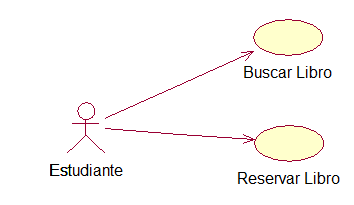
\includegraphics[width=10cm]{./Imagenes/img1} 
	\end{center}
	
	\begin{center}
	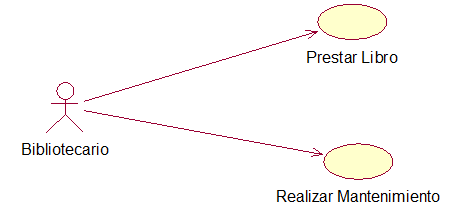
\includegraphics[width=10cm]{./Imagenes/img2} 
	\end{center}

\end{enumerate} 

\section{ DISEÑO (Diagrama de Clases, Modelo Entidad Relacion)} 

\begin{enumerate}[1.]
	\item Diagrama de Clases, Modelo Entidad Relacion.
    


	

	\begin{center}
	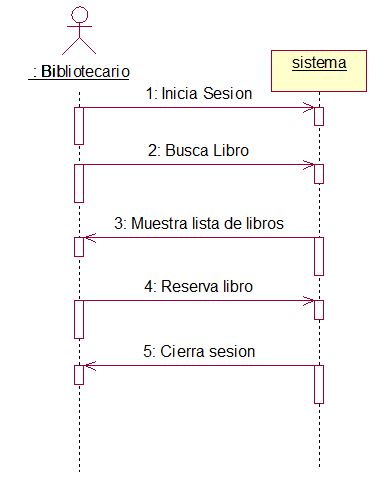
\includegraphics[width=10cm]{./Imagenes/img5} 
	\end{center}
	
	\begin{center}
	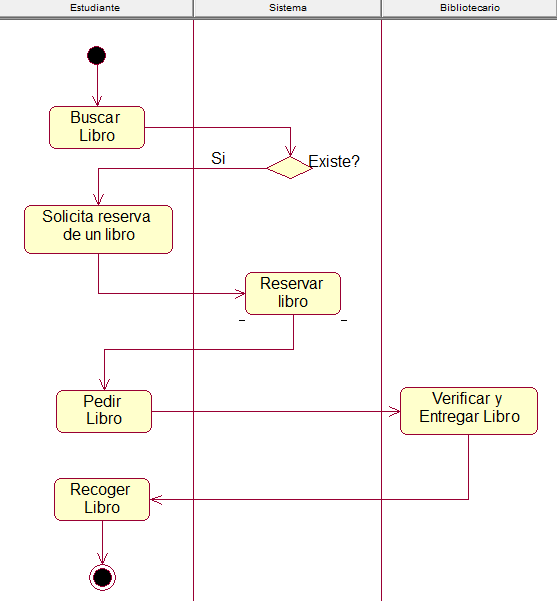
\includegraphics[width=10cm]{./Imagenes/img6} 
	\end{center}
	
	\begin{center}
	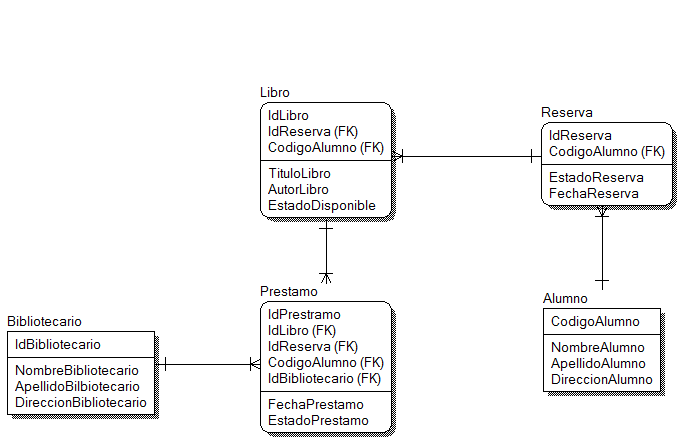
\includegraphics[width=20cm]{./Imagenes/img8} 
	\end{center}
	
	
\end{enumerate} 

\section{ DISEÑO INTERFAZ DE USUARIO (Pantallas y metodos de clases utilizados)} 
  \subsection{Clase alumno}
  La clase alumno en esta clase esta la informacion necesaria de un alumno para poder participar como usuario de la biblioteca.
	\begin{center}
	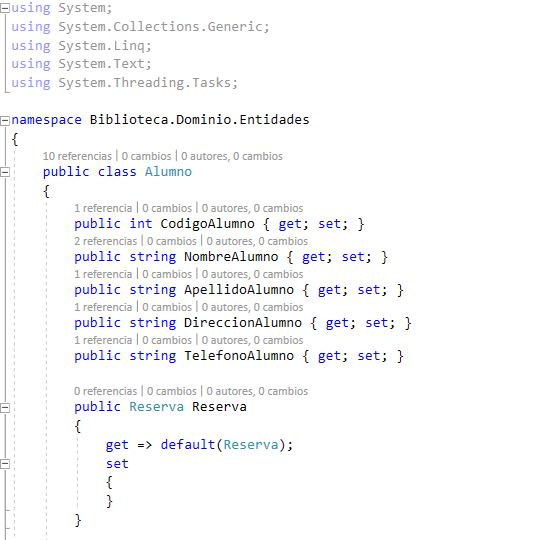
\includegraphics[width=14cm]{./Imagenes/img101} 
	\end{center}

	
	
 \newpage
 \subsection{Clase libro}
 Dentro de la clase libro encontramos los datos necesarios e infromacion de un libro para poder regitrar en una bilbioteca
 	\begin{center}
	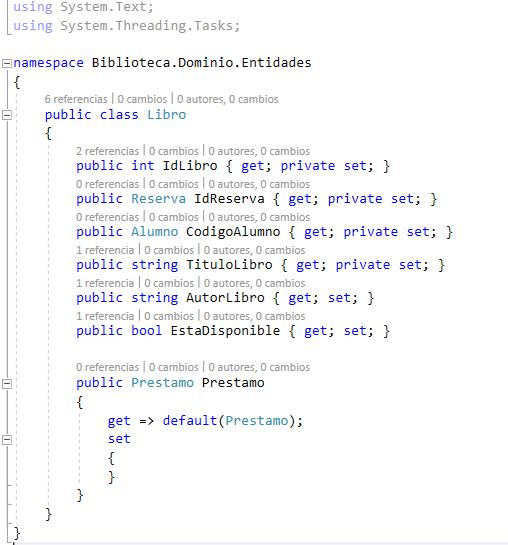
\includegraphics[width=12cm]{./Imagenes/img11libro} 
	\end{center}
	
 \newpage
 \subsection{Clase prestamo}
 Dentro de la clase prestamo encontramos los datos necesarios para realizacion de un prestamos de libro ya sea la fecha la hora y demas datos del alumno que realiza el prestamo y como tambien del bibliotecario.
 	\begin{center}
	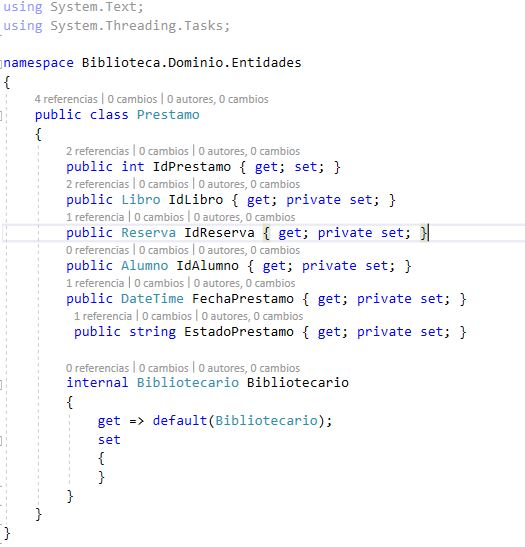
\includegraphics[width=14cm]{./Imagenes/img12prestamo} 
	\end{center}
	
	
 \newpage
 \subsection{Clase Reserva}
 Dentro de la clase resreva encontramos los datos necesarios para realizacion de una reserva de libro como que libro se prestara, su estado entre datos importantes que necesitamos para eralizar la reserva.
 	\begin{center}
	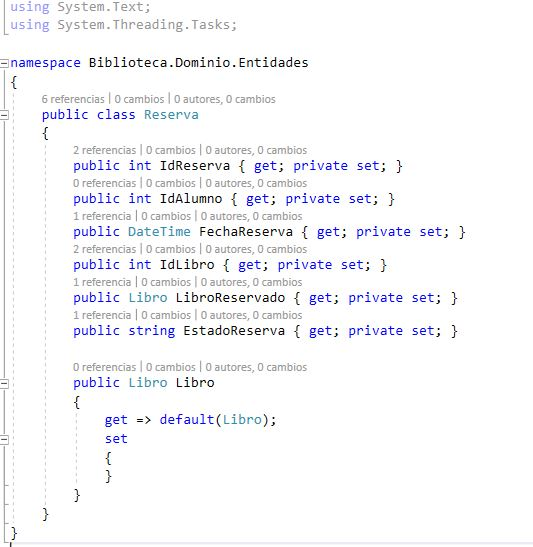
\includegraphics[width=14cm]{./Imagenes/img13reserva} 
	\end{center}
	
 \newpage
 \subsection{Clase Bibliotecario}
 Dentro de la clase  bibliotecario se encuentran los datos del biblbiotecario quien usara el sistema al momento de realizar los prestamos .
 	\begin{center}
	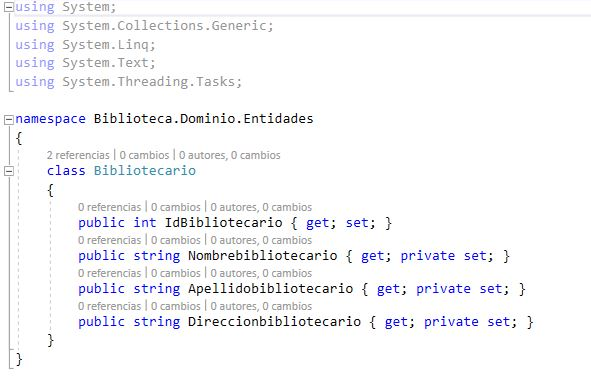
\includegraphics[width=14cm]{./Imagenes/img11bibliotecario} 
	\end{center}


\end{document}
